\chapter{Source Cleaning Apparatus Manual}
\section{Purpose}
This document describes the necessary information and standard procedures that \textbf{must} be followed for the operation and handling of  the source cleaning vessel. In case a part or step of this procedure is not clear or a statement in the procedure contradicts the state of experiment, do not continue with the process. Contact the calibration coordinator and detector manager and get permission to proceed 
\section{Definitions}
\textbf{Cleaning Module}: An apparatus that can be attached directly to the source tube gate valve that sprays a flow of LAB directly onto a source to facilitate cleaning. The set up allows to draw LAB for testing .\\
\\
\textbf{Source Connector}:A device by which a source may be temporarily connected to an umbilical while also allowing bre optic or electrical connections.\\
\\
\textbf{Umbilical Retrieval Mechanism(URM)}:The device in which the umbilical is stored
in preparation for deployment that also includes drive mechanisms for the central rope and umbilical to facilitate vertical movement of sources.\\
\\
\textbf{Source Tube}: A tube connecting to the bottom of the URM with a bellows below that terminates on a gate valve that connects to a nipple assembly on the UI when the URM is in a position ready for deployment.\\
\\
\textbf{Umbilical}: A length of Tygothane tubing containing an optical fiber and five electrical wires to which calibration sources are attached for deployment in the AV.\\
\\
\textbf{Boil Off Nitrogen}: Nitrogen sourced from a cryogenic nitrogen dewar that is installed in the Utility drift and is transferred  to the DCR by way of copper conduit (high pressure) or from the international dewar (low pressure). The pressure of the high pressure nitrogen boil off  for purging purposes must be regulated using the gas board in the DCR to less than 20 psi. ( @ Ryan Reference to the relevant procedure required )\\
\\
\textbf{Linear Alkyl Benzene(LAB) cleaning set up}: This setup is designed to clean the LAB. The complete unit consists of different parts such as pump, filters, pulsation dampener, piping system, fitting and cart.\\
\section{Description of the Cleaning Module}
The cleaning module consists of a  31.78" long cylindrical tube with 9.50" interior diameter. Inlet and outlet gas connections are supplied to allow nitrogen flushing of the module independent of the URM system. Four LAB sprayers near the top of the cleaning module provide a stream of LAB to actively rinse the source. The flange at the top of the source allows  to connect the cleaning module to the gate valve at the bottom of the URM source bellows. A cart with a jack is provided to move and lift the cleaning module into position, and provide a clean working surface for source work.
\begin{figure}[!htpb]
  \centering
  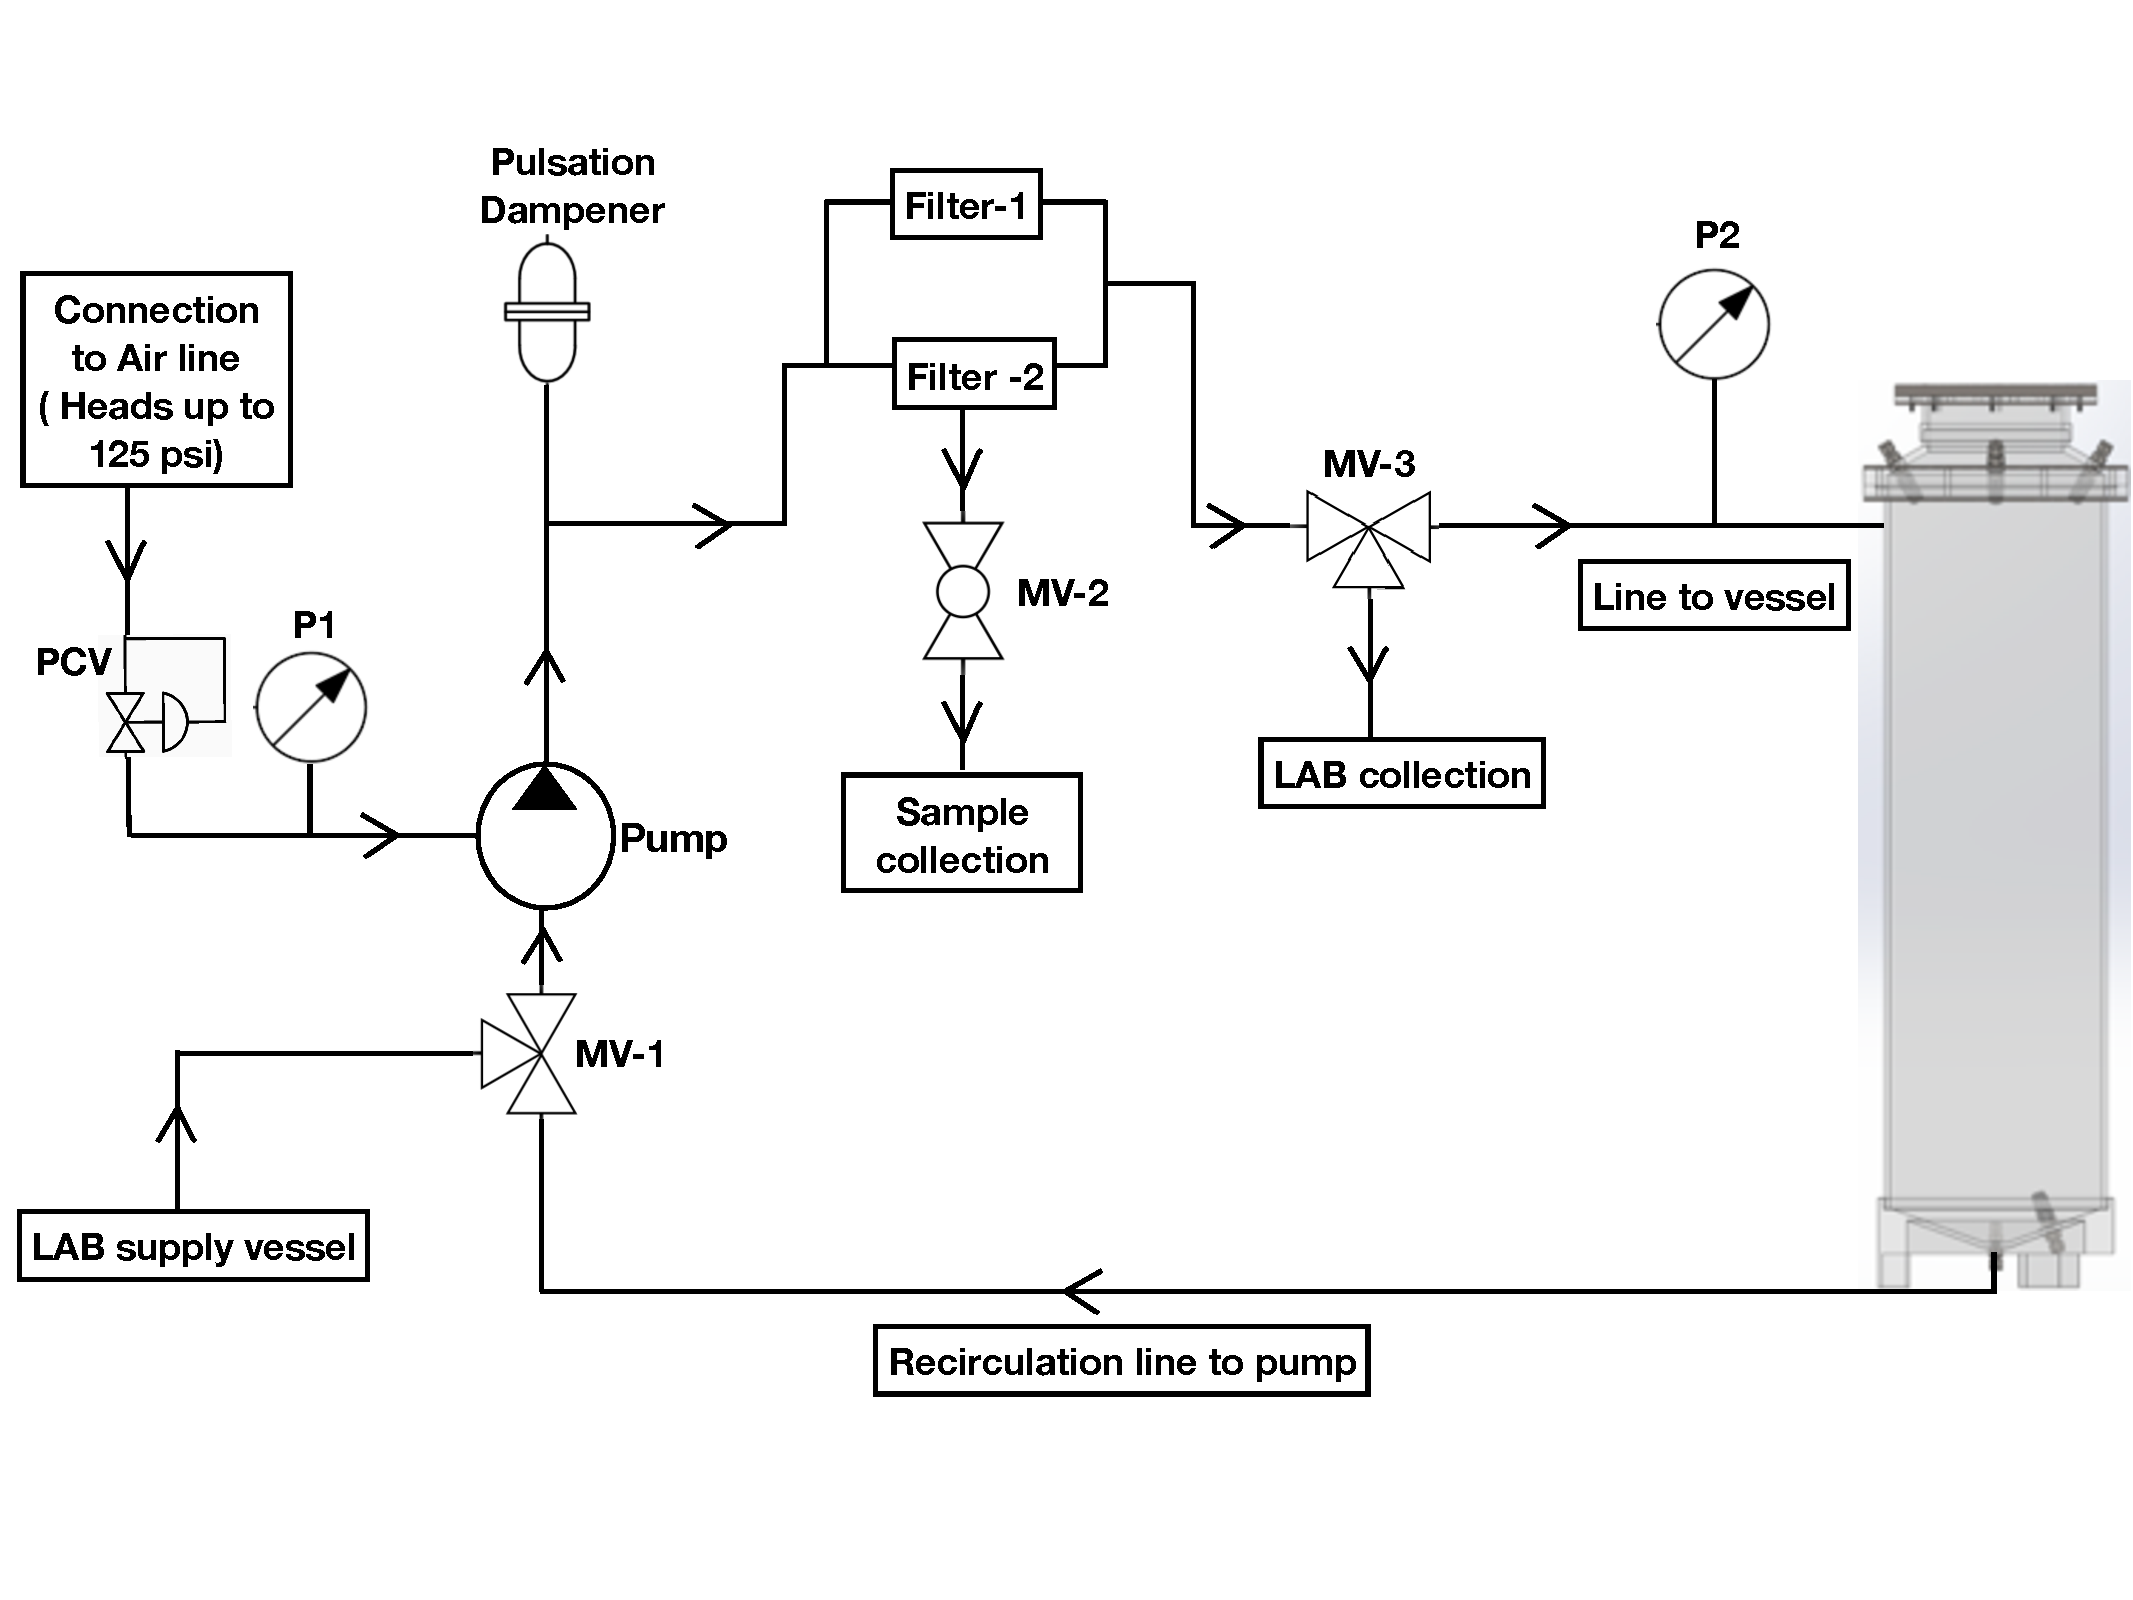
\includegraphics[width = 14cm, height=14cm ]{figures/LAB_3}
  \caption{Line Diagram of the LAB cleaning set up}
  \label{fig:SCV}
\end{figure}
\\
\section{Important points and prerequisite}
Before commencing any activities related to the source cleaning vessel and LAB set up, the designated people should follow these steps:
\begin{enumerate}
\item The Safety Data Sheet (SDS) must be thoroughly reviewed each time when handling LAB. Permission from the detector manager must be obtained in writing.
\item All person must be equipped with required PPE ( Nitrile gloves, masks, safety glasses, head cap) before the starting of any procedure and change them as required.
\item The vessels must be handled with fresh, clean gloves and face masks must be used by the individuals involved in the activity.
\item  When moving the vessels, there must be at least three people present: one will be the “dirty” person, the other two “clean”.
\item The “dirty” person must keep an eye on the clean persons at all time and ensure that the clean persons not get in contact with any unclean surface.  If in any case it happen then instruct them to change their PPE.
\item Every piece of equipment that will receive parts or need additional items like wrenches, screw drivers etc. need to be set up first (checked, cleaned and put in appropriate location etc) before the vessel is moved, or used.
\item The receiving parts must be thoroughly cleaned with Ultra Pure Water(LPW). 
\item No clean part should be touched without clean gloves and masks on.

\end{enumerate}


\section{Procedures}
The following procedures must be done within the deck clean room and all necessary protocols must be followed. It is assumed that the operator is to perform all operations using latex gloves in addition to standard Personal Protective Equipment (PPE). Dust counts should be monitored prior to operations involving opening the  URM source tube or exposing a source. If the dust count appears to be high, the DCR should be cleaned and the intended procedure should be suspended. All procedures listed here should be completed with the participation of a calibration expert.

\subsection{Connecting the URM to the UI}

\subsection{Disconnecting the URM from the UI}

\subsection{Using the Source Connector}

\subsection{Attaching a Source to the Umbilical}\label{ss:sourceattach}

 The instructions below presuppose that the source is not connected to the umbilical. Note that the following only applies to the North side URM as the South side URM will have the Cherenkov source permanently attached to its umbilical. Sources of LAB, and boil off nitrogen should be procured before attempting the following procedure.

\begin{enumerate}
\item Begin with the source in the cleaning module
\item Start the flushing the cleaning module with N$_{2}$ 
\item Move the URM back from the UI over the working area West of the UI
\item Position the cleaning module cart under the URM
\item Close the URM cover gas bag and start actively flushing the URM with N$_{2}$
\item Open the gate valve and lower the source connector until it can reach the source.
\item Connect the source to the umbilical via the source connector. 
\item Raise the source into the source tube
\item Connect the cleaning module to the source tube gate valve
\item Make connections (Can be done by any one of the two clean person) for the  airline fitting at the specified port on the  LAB cleaning set up for starting the pump.
\item Check the connection for the inlet of LAB cleaning set up with LAB supply vessel (Ensure that the vessel  is filled with the minimum level (approximately 10 litre) of LAB required for the cleaning procedure ).
\item Set the bottom MV1  toward the injection line and the MV3 toward  line to the vessel.
\item Start the pump by providing the pressure from the Air line ( Maximum upto 125 psi, Pressure can be controlled by the pressure control valve) and allow LAB to flow in the LAB cleaning set up.
\item Wait until an adequate amount (When a 2/3 volume of the bottom conical part in the source cleaning vessel is filled with the LAB) of LAB is pumped in the LAB cleaning set up.
\item Once the adequate amount of LAB is filled  in the LAB cleaning set up then stop the pump and set the MV1 toward the recirculation line.
\item Turn on the pump again and allow LAB to flow in the LAB cleaning set up.
\item While the LAB flowing  lower the source through the LAB stream. The source should be  raised and lowered through the spray to remove surface contamination. The initial rinse should continue until the source (and the source connector) are clean.
\item Monitor the O$_2$ levels in the URM to validate the cover gas viability. The URM radon levels should also be monitored directly using the RAD7. The cover gas should be considered viable after the measured radon levels are consistent with zero. Once the cover gas is deemed viable the N$_{2}$ flush can be terminated and the cover gas bags can be opened to the URM. 
\item Take a sample to be submitted for analysis. To collect samples, set the manual MV2 at the On position, after collecting samples set the valves again at the off position.
\item Repeat spraying the source with LAB as above until the source get sample analysing . Allow the source to sit in the LAB for some time (order of a week) periodically draining the LAB, submitting samples for analysis . Record the status of the LAB cleanliness for each sample preparation (need to define a quantifiable cleanliness criteria)
\item Once the LAB cleanliness criteria is reached (TBD) the source should be raised into the source tube, the gate valve closed and the cleaning module disconnected from the gate valve. 
\item Move the URM back to the UI and reconnect the gate valve to the nipple assembly on the UI
\item Once the cleaning operation is complete, then the remaining LAB from the processing lines can be flushed out from the LAB cleaning set up by using the “dump” line. 
\item To do this, again turn off the pump, set the MV3 to the “dump” line where it should be connected to a container to accumulate the fluid. 
\item Then turn the pump on and pump until there is no more fluid exiting the dump line. Note that this will remove the majority of the fluid, but there will always be some fluid left within the process lines. 
\item Turn off the pump by stopping the pressure from the Air line at the specified port. 
\end{enumerate}

\subsection{Cleaning a Source Prior to Use}
Here, the minimum guidelines for cleaning a source should be set out. Each group should have their own specific cleaning instructions which should be compiled with this document. However, prior to use each source should
\begin{enumerate}
\item be inspected by a designated person to look for signs of corrosion or damage to the source
\item be wiped down using ultra pure water to initially pick up surface contaminants
\item be wiped down with an alconox mixture to futher remove surface contaminants
\item be wiped down with ultra pure water again to remove the alconox
\end{enumerate}

\subsection{Detaching a Source from the Umbilical}
Required for this procedure is a storage module for the source. This module should be connected to a pump/purge system to keep the source in a nitrogen environment between uses.
\begin{enumerate}
\item Ensure that the source storage module is available for use on the source cart.
\item Disconnect the URM from the UI.
\item Move the URM back to the working area and place the source cart in the working area
\item Disconnect the URM cover gas bag and flush nitrogen through the URM.
\item Open the source tube gate valve over the working surface of the source cart.
\item Lower the source to the working surface of the source cart.
\item Disconnect the source from the umbilical at the source connector.
\item Place the source in the storage module. Close the storage module and pump nitrogen into the storage module.
\item If a new source is not to be immediately connected to the umbilical, retract the source connector back into the URM source tube and close the gate valve. Continue the URM purge until O$_{2}$ monitor and RAD7 values are below established thresholds before the cover gas bags are reconnected. 
\item If a new source is to be reconnected refer to Section \ref{ss:sourceattach}.
\end{enumerate}




